% \documentclass{standalone}
% \usepackage{pgfplots}
% \pgfplotsset{compat=1.17}
% \begin{document}
%
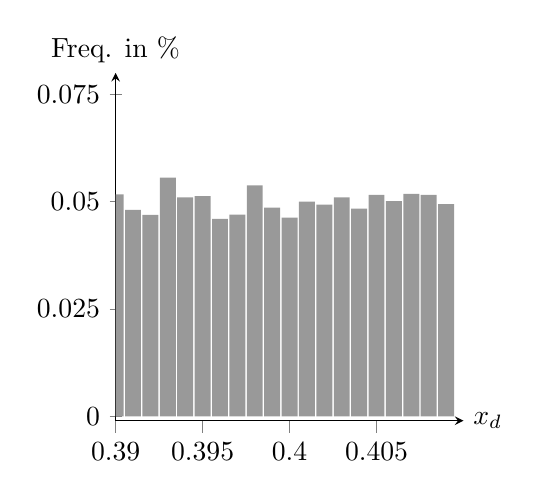
\begin{tikzpicture}

    \begin{axis}[
        width=6cm,height=6cm,
        axis lines=left,
        scaled y ticks=false,
        ylabel={Freq. in \%},
        xlabel={$x_d$},
        every axis y label/.style={at={(current axis.north west)},above=0mm},
        every axis x label/.style={at={(current axis.south east)},right=0mm},
        ybar=0pt,
        bar width=5.75pt,
        ymin=-0.001,
        ymax=0.080,
        ytick={0, 0.025, 0.05, 0.075},
        yticklabels={$0$, $0.025$, $0.05$, $0.075$},
        xmin=0.39,
        xmax=0.41,
        xtick={0.39, 0.395, 0.4, 0.405},
        xticklabels={$0.39$, $0.395$, $0.4$, $0.405$},
    ]
    \addplot[draw opacity=0.0, fill=black!40]
        coordinates {
            (0.3900009, 0.05169)
            (0.3910007, 0.04810)
            (0.3920006, 0.04690)
            (0.3930004, 0.05560)
            (0.3940003, 0.05100)
            (0.3950001, 0.05130)
            (0.3960000, 0.04600)
            (0.3969998, 0.04700)
            (0.3979997, 0.05380)
            (0.3989995, 0.04860)
            (0.3999994, 0.04630)
            (0.4009993, 0.05000)
            (0.4019991, 0.04930)
            (0.4029990, 0.05100)
            (0.4039988, 0.04840)
            (0.4049987, 0.05160)
            (0.4059985, 0.05010)
            (0.4069984, 0.05180)
            (0.4079982, 0.05160)
            (0.4089981, 0.04940)
            };
    \end{axis}
\end{tikzpicture}

% \end{document}